\documentclass{article}
\usepackage{polski}
\usepackage[utf8]{inputenc}
\usepackage{hyperref}

\usepackage{graphicx}
\graphicspath{ {./assets/} }
\hypersetup{
    colorlinks,
    citecolor=black,
    filecolor=black,
    linkcolor=black,
    urlcolor=black
}

\title{
    WMI Adventure - grywalizacja studiowania Informatyki \\
    \large Zarządzanie projektem i metodyka zwinna
    }
\author{Marcin Kostrzewski}
\date{22 Listopada, 2021r}

\begin{document}

\maketitle
\newpage
\tableofcontents
\newpage


\section{Wstęp}

\subsection{Streszczenie}
Zarządzanie projektami informatycznymi zaczęło mnie interesować już na 3 roku studiów, gdzie miałem przyjemność uczestniczyć w zajęciach z Inżynierii Oprogramowania prowadzonych przez
dr. Krzysztofa Krzywdzińskiego, w grupie zajęciowej u dr. Patryka Żywicy. WMI Adventure, będący pierwszym większym projektem który realizowałem drużynowo, byłem w dużym stopniu odpowiedzialny za
proces który implementowaliśmy.

Napisałem tę pracę korzystając ze zdobytej wcześniej wiedzy między innymi na zajęciach uczelnianych, z przeczytanych książek,
oraz z doświadczenia zdobytego podczas WMI Adventure. Omawiam w niej różne metodyki zwinne, porównuje je do dawnego, kaskadowego podejścia przedstawiając ich tło historyczne. Przedstawiam też cały proces w WMI Adventure, wykorzystaną metodykę i narzędzia wspomagające.

\subsection{Tematyka}
W zespołach organizacja pracy projektowej jest kluczowa dla kontrolowanego i przewidywalnego rozwoju, w tym przypadku, oprogramowania komputerowego. W systemach o mniejszym stopniu skomplikowania
i jednoosobowej sile roboczej wystarczy "tylko programowanie". W miarę poszerzania skali projektu i zwiększania ilości członków zespołu, wytwarzanie oprogramowania staje się chaotyczne i niekontrolowane.

Klient, dla którego realizowany jest projekt potrzebuje wspomnianej przewidywalności. Chce chociażby wiedzieć, ile czasu potrwa realizacja jego zlecenia i przede wszystkim jaki będzie jego koszt. Zespół nie jest w stanie
rejestrować postępu prac. Każdy z członków ma inną wizję projektu i priorytetuje zupełnie inne rzeczy, niż te, które są faktycznie istotne dla klienta. Nie wiadomo, nad czym zespoł w danej chwili pracuje.

Potrzeba zatem pewnej struktury, która sprawi, że rozwój oprogramowania będzie przewidywalny - tym właśnie jest zarządzanie projektem, a metodyki to zbiór pewnych ram, które ułatwią jego rozwój.

\subsection{Cel}
WMI Adventure było piaskownicą, którą wykorzystałem do nauki zarządzania zespołem w praktyce. Analizując skutki które przynosiły moje (i innych członków zespołu) decyzje, starałem się z każdym tygodniem usprawniać
proces, wynosząc przy tym doświadczenie i  wiedzę, którą chcę tutaj przekazać.

W litetaturze czy materiałach dostępnych w internecie możemy znaleźć ogólne zasady zarządzania projektem, które też tutaj przytaczam, natomaist
meritum pracy znajduje się w opisie konkretnego wykorzystania tych zasad w oparciu o WMI Adventure, które omawiam w jej drugiej części.

Drużyna WMI Adventure liczyła początkowo 4 członków, końcowo trzech. Koordynacja mniejszymi zespołami wcale nie musi być prostsza niż tymi dużymi. Chcę w tej pracy opisać metodyki w oparciu o małe zespoły i dostarczyć informację na temat problemów i potencjalnych rozwiązań, które w takich drużynach
występują.

\section{Metodyki pracy i ich kontekst historyczny}
Metodyka pracy to pewien zbiór zasad, które określają w jaki sposób zespoł ma realizować swoje cele. Droga do osiągnięcia tych celów jest skomplikowana i wymaga koordynacji i zarządzania. Metodyka odpowie nam na takie pytania jak: Jaką strukture ma tworzyć zespół? Na jakie role podzielony jest zespół i jakie są odpowiedzialności poszczególnych ról? Jak mierzyć postęp w projekcie? Jak zbierać wymagania projektowe od klienta? Jak wygląda cykl życia projektu? W jaki sposób zarządza się ryzykiem?

Wybór metodyki ma zatem ogromny wpływ na pracę zespołu - sposobów na zrealizowanie jednego celu może być nieskończenie wiele, każdy ma swoje konsekwencje i może doprowadzić do jego pomyślnego ukończenia, lub do całkowitej porażki. Przypadek, w którym nie zastosujemy żadnych schematów i będziemy po prostu programować według własnych zasad też jest w pewnym sensie metodyką, wcale nie skazaną na porażkę.

Metodyka pracy mówi nam zatem \textit{jak} wytwarzać oprogramowanie.

\subsection{Metodyki kaskadowe}
Początki korporacyjnego świata projektów informatycznych wykorzystywały metodykę kaskadową. Metodyki te mogły wywodzić się z doświadczenia inżynieryjnego zdobytego w fabrykach.\footnote{M. Chrapko - Scrum - o zwinnym zarządzaniu projektami, 2015, Helion, s. 27} Linia produkcyjna w fabryce jest
stałym elementem i nie jest odporna na zmiany. Półprodukt przechodzi z jednej linii do drugiej. Nie ma możliwości, żeby gotowy przedmiot opuścił fabrykę bez przejścia każdego etapu bez jakiejkolwiek porażki.
Każdy błąd popełniony przez pracowników na linii produkcyjnej jest katastrofalny i nie jest tolerowany.

Metody kaskadowe w projektach informatycznych działają podobnie - drużyna nie jest przystosowana na zmiany, zakładane jest, że wymagania projektowe nigdy się nie zmienią i żadne błędy nie zostaną popełnione na danych etapach projektu. Poszczególne fazy projektu realizowane są sekwencyjnie - jeden po drugim, co skutkuje tym, że błędy z wcześniejszych faz są propagowane na kolejne - często ich magnituda rośnie eksponencjalnie z każdym kolejnym etapem.

Drużyny w takich metodykach często składają się dużej liczby członków odpowiedzialnych za konkretne, zdefiniowane czynności.

Przykładem metodyki kaskadowej jest \textbf{Rational unified process (RUP)}

\subsubsection{Cykl życia projektu - Wodospad}
\begin{center}
    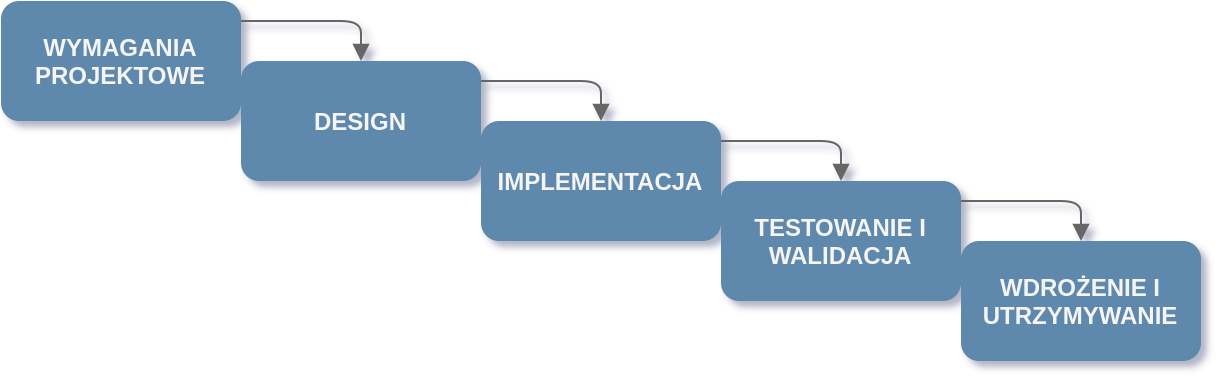
\includegraphics[scale=0.25]{waterfall_diagram.png}
\end{center}

\subsubsection*{Wymagania projektowe}
Główna faza kontaktu z klientem. Analitycy zbierają wymagania od klienta i decydują, czy projekt zostanie zrealizowany. Szacowany jest jego czas trwania i koszt. Wynikiem końcowym tego etapu są często pierwsze dokumenty opisujące funkcjonalności w systemie - \textbf{Use cases - przypadki użycia} i \textbf{Dokument wizji projektu}

Dokument wizji projektu odpowiada na pytanie \textit{Jak będzie wyglądał projekt i jaką wartość dostarczy klientowi}. Zawierają się w nim między innymi cele projektu - jak rozwiązać \textit{problem} - czyli czego klient tak naprawdę potrzebuje, opisuje grupę odbiorców systemu, produkt końcowy i wartości które wniesie. Definiowany jest zakres systemu.

Przypadki użycia - use cases to szczegółowe opisy konkretnych funkcji w systemie opisane w formie ścieżek, jakie dany odbiorca będzie przechodził, żeby osiągnąć konkretny dla niego cel. Use cases są bardzo szczegółowe i przedstawiają wszystkie możliwe ścieżki i zachowania systemu.

Przykładowy Use Case utworzony przeze mnie na potrzeby kursu z \textit{Inżynierii oprogramowania}:

\subsubsection*{Kontekst: System zarządzania projektami w firmie produkującej filmy wideo}
\subsubsection*{Use Case: Wprowadzenie projektu do systemu}
\textbf{Aktor podstawowy: \textit{Szef firmy}}

\subsubsection*{Główni odbiorcy i oczekiwania względem systemu}
\begin{itemize}
    \item Szef: jest to podstawowa funkcja z jakiej szef będzie korzystał. Zależy mu na tym, aby dostęp do niej był szybki. Chce, aby wprowadzanie danych o projekcie było objęte pewnymi stałymi ramami, do których interfejs będzie dostosowany.
    \item Pracownik: oczekuje dostępu do nowego projektu wraz ze wszystkimi istotnymi informacjami o nim
    \item Klient: nie chciałby, aby musiał podawać dane kilkakrotnie, powinien mieć możliwość otrzymania informacji o stanie jego projektu
    \item Przedsiębiorstwo: potrzebuje dobrej organizacji wszystkich projektów, systematyzowania danych i ich bezpieczeństwa. W przypadku awarii systemu bądź sprzętu, musi mieć możliwość odzyskania krytycznych danych
\end{itemize}

\subsubsection*{Warunki wstępne}
Szef jest zalogowany w systemie i ma dostęp do interfejsu zarządzania zadaniami. Baza danych ma wystarczającą ilość przestrzeni
dyskowej, aby mógł zostać dodany wpis o projekcie.

\subsubsection*{Warunki końcowe}
Baza danych jest zaktualizowana o wpis z wszystkimi koniecznymi informacjami o projekcie. Ustalana
jest data wprowadzenia projektu do systemu, generowany jest wpis w historii. Na osobnym dysku tworzona jest
kopia zapasowa z wpisem do bazy. Projekt jest widoczny na tablicy pracowników i tablicy szefa. System jest w
gotowości do przydzielenia ról i zadań pracownikom.

\subsubsection*{Scenariusz główny}
\begin{enumerate}
    \item Podczas rozmowy z klientem, szef otwiera moduł tworzenia projektu na swoim komputerze PC poprzez aplikacę webową
    \item Szef wprowadza dane o projekcie, wypełnia konieczne pola, między innymi: nazwę projektu, typ, krótki opis i zatwierdza utworzenie.
    \item Po zatwiedzeniu wyświetlane są wprowadzone dane w zwizualizowanej postaci (tabela)
    \item Szef ma możliwość modyfikacji lub zatwierdzenia projektu \newline \textit{W przypadku modyfikacji, powtarza krok 2 i 3}
    \item System przekazuje dane z klienta do serwera. Tworzony jest nowy wpis w bazie danych oraz kopia zapasowa.
    \item Na aplikacjach klienckich wyświetla się powiadomienie o nowym projekcie.
    \item Szef otrzymuje wiadomość zwrotną, że projekt został dodany pomyślnie
    \item W dowolnym momencie może zostać wprowadzana zmiana w danych projektu, mogą zostać załączone zewnętrzne dokumenty. \textit{Powtarzane są wtedy kroki 2-4}. Wpis w bazie danych oraz kopia zapasowa są aktualizowane.
\end{enumerate}

\subsubsection*{Rozszerzenia}

\subsubsection*{* W dowolnym momencie system ulega awarii}
Integralnośc danych musi zostać zachowana, zatem konieczna jest transakcyjność. Aktualizacje
i tworzenie wpisów o projekcie musi zostać zaktualizowane tylko w przypadku kompletnego przesłania
danych z aplikacji klienckiej do serwera i bazy danych
\begin{enumerate}
    \item W przypadku automatycznego powrotu systemu do stanu gotowości, szef sprawdza, czy wpis o nowym projekcie został utworzony
          \begin{enumerate}
              \item W przypadku braku wpisu, proces dodania projektu jest powtarzany
              \item W przypadku poprawnego dodania wpisu, proces przebiega pomyślnie i szef może kontynuować pracę
          \end{enumerate}
    \item Gdy system nie powraca do stanu gotowości, szef musi poinformować administratora o błędzie w systemie. Administrator podejmuje odpowiednie kroki, aby przywrócić system do działania
\end{enumerate}

\subsubsection*{2. Niekompletne dane}
W przypadku, gdy nie zostanie wprowadzona \textit{nazwa projektu}, projekt nie zostanie dodany, szef zostanie poinformowany o błędzie.

\subsubsection*{5a. Błąd połączenia z serwerem lub błąd bazy danych}
Wpis o nowym projekcie nie zostaje dodany. Aplikacja kliencka informuje o błędzie połączenia z serwerem i konieczności skontakowania się z administratorem

\subsubsection*{5b. Projekt już istnieje}
Gdy system bazodanowy wykryje, że projekt o tej samej nazwie istnieje już w bazie, wpis o nim nie jest dodawany. Interfejs sygnalizuje o błędzie i konieczności zmiany nazwy projektu.

\subsubsection*{8a. Błędnie wprowadzone dane}
Gdy system wykryje, że np. zmieniana jest nazwa projektu na nazwę już istniejącą, zwróci błąd.

\subsubsection*{8b. Załączanie plików}
Szef może chcieć dodać dokument do projektu.
\begin{enumerate}
    \item Interfejs graficzny oferuję przesłanie i tym samym załączenie pliku do projektu.
    \item Szef wybiera plik i przesyła go na serwer.
          \begin{enumerate}
              \item Obliczana jest ilość wolnego miejsca na dysku serwerowym. Gdy ilość wolnego miejsca nie jest wystarczająca do przesłania pliku, zostaje zwrócony błąd.
              \item Podczas przesyłania występuje zerwanie połączenia. Plik nie jest przesłany i zostaje wysłane powiadomienie do aplikacji klienckiej.
              \item Gdy plik jest wysłany poprawnie i znajduje się już na serwerze, tworzona jest jego kopia zapasowa, oraz dodawany jest wpis w bazie danych zawierający ścieżkę do dokumentu.
              \item W przypadku sukcesu wszystkich procesów, zwracana jest wiadomość o sukcesie
          \end{enumerate}
\end{enumerate}

\subsubsection*{Design}
Na podstawie wcześniej zebranych wymagań analitycy we współpracy z architektami systemu decydują jak będzie wyglądał końcowy efekt i w jaki sposób zostanie utworzony. Podejmowane są tutaj takie decyzje jak wybór technologii i achitektura całego systemu, tworzone są wstępne projekty intefrejsu. Po tej fazie wszystkie Use Case'y dla projektu powinny zostać ukończone. Powstaje także \textbf{dokument wymagań projektowych} stanowiący bardziej techniczną i szczegółową wersję dokumentu wizji. Definiowany jest zakres systemu, wymagania funkcjonalne i niefunkcjonalne czy kryteria akceptacji i ryzyka projektowe.

\subsubsection*{Implementacja}
Zespół programistów ze współpracy z architektami systemu implementują jego design. W tej fazie powinna powstać większość bytów programistycznych realizująca cały zakres systemu.

\subsubsection*{Testowanie i walidacja}
Po ukończeniu prac programistycznych zespół odpowiedzialny za testowanie systemu rozpoczyna swoją pracę i sprawdza, czy cały system działa. Implementacja jest weryfikowana pod kątem spełnienia wymagań projektowych, tworzone są raporty z testów, ostatnie funkcjonalności są zaimlpementowane. Wszystkie use casy są zrealizowane.

\subsubsection*{Wdrożenie i utrzymanie}
System jest przygotowywany do oddania klientowi. Administratorzy systemowi wdrażają cały projekt według zaplanowanego rozwiązania architektonicznego. Tworzone są dokumenty instruujące jego odbiorców jak go używać.

Po wdrożeniu system jest dalej utrzymywany według wcześniej ustalonych zasad, poprawiane są błędy, które wcześniej nie zostały wykryte. System nie powinien być już dalej uzupełniany o nowe funkcjonalności.

\subsection{Agile}
Agile to rodzina metod, która zaczęła rozwijać się na przestrzeni lat 80-tych i 90-tych ubiegłego stulecia jako opozycja starego podejścia metodyk kaskadowych\footnote{M. Chrapko - Scrum - o zwinnym zarządzaniu projektami, 2015, Helion, s. 33}, jako, w pewnym sensie, nauka na błędach. Deweloperzy byli zmęczeni wielkimi korporacyjnymi strukturami stojącymi za kaskadowym procesem, które tłumiły wszelkie indywidualne inicjatywy na rzecz "decyzji z góry". Kreatywność nie była cechą cenioną. Programiści nie musieli myśleć - ich zadaniem było realizowanie architektury zaplanowanej przez architekta. Nikt nie zastanawiał się nad tym, czy zadania im powierzone mają sens.

Agile jest w pewnym sensie procesem odwrotnym do metodyk kaskadowych\footnote{M. Chrapko - Scrum - o zwinnym zarządzaniu projektami, 2015, Helion, s. 31}. Wodospad, czyli jeden etap po drugim - w Agile wszystkie etapy dzieją się tak naprawdę jednocześnie. Stały schemat metody pracy i brak reakcji na błędy został zastąpiony ciągłymi zmianami i budowaniem procesu w oparciu o niepowodzenia. Ba, zmiany stały się nieodłączną częścią całego procesu. Kontakt z klientem jest bardzo częsty i aktywny przez cały. Indywidualne inicjatywy członków zespołu budują cały proces. Nowe funkcjonalności systemu są testowane na bieżąco. Metodologie Agile idealnie podsumowuje \textbf{Manifest Agile (Agile Manifesto)}

\subsubsection{Manifest Agile}

\begin{center}
    Ludzie i interakcje ponad procesami i narzędziami

    Działające produkty ponad złożoną dokumentacją

    Współpraca z klientem ponad negocjacją kontraktu

    Reagowanie na zmiany ponad trzymaniem się planu\footnote{M. Chrapko - Scrum - o zwinnym zarządzaniu projektami, 2015, Helion, s. 34}
\end{center}

\subsubsection*{Ludzie i interakcje ponad procesami i narzędziami}
Największy wpływ na rozwój projektu mają właśnie ludzie - to dzięki ich kreatywności i zaangażowaniu skomplikowana maszyna projektowa idzie do przodu. Narzucanie ścisłych zasad procesowych ogranicza możliwości zespołu, a skomplikowane narzędzia wcale nie ułatwiają im pracy.

\subsubsection*{Działające produkty ponad złożoną dokumentacją}
Tutaj mowa o wspomnianym wcześniej podejściu odwrotnym do wodospadu - wytwarzając skomplikowane oprogramowanie jako jedną całość tracimy możliwość wprowadzania zmian w trakcie projektu - Agile mówi, żeby poszczególne etapy projektu były małe i kończyły się jakąś działającą częścią systemu. Dzięki temu możemy raportować klientowi postępy pracy i łatwo dostosowywać się do jego uwag czy sugestii. Inkrementacyjne wytwarzanie oprogramowania umożliwia też stałe testowanie i bardziej realistyczne określanie dalszych ryzyk w projekcie.

\subsubsection*{Współpraca z klientem ponad negocjacją kontraktu}
W modelu kaskadowym wkład w projekt klienta był tak naprawdę znikomy. Na początku projektu podczas zbierania wymagań decydowano tak naprawdę czy projekt ma sens, czy nie. Zespół obawiał się wszelkich zmian ze strony klienta po zatwierdzeniu wymagań. W Agile klient jest stale zaangażowany w rozwój projektu. Wymagania zawsze mogą ulegać zmianie i iteracyjny rozwój oprogramowania jest na nie otwarty. Satysfakcja klienta również jest dużo wyższa, stałe postępy w pracy nad projektem są dla niego widoczne.

\subsubsection*{Reagowanie na zmiany ponad trzymaniem się planu}
Nie pracowałem nigdy w projekcie, w którym wszystko wychodziłoby tak, jak zostało to na początku zaplanowane. W Agile zespół powinien być stale otwarty na pojawiające się zmiany i dostosowywać swoje zmiany pracując razem z nimi.

\paragraph{}
Metody wodospadowe były określane jako "powtarzalne"\footnote{M. Chrapko - Scrum - o zwinnym zarządzaniu projektami, 2015, Helion, s. 31}, bo każdy projekt realizowany był w bardzo podobny sposób. W Agile można zaobserwować "odwrotne" podejście - każdy projekt należy traktować w inny sposób. Specyfika każdego projektu może decydować o tym jak będzie wyglądała praca zespołu. Sam zespół składa się z ludzi, których zachowania i charaktery wcale nie są powtarzalne, jak to zakładało podejście kaskadowe. Każdy projekt realizowany zwinnie ma w pewnym sensie swojego własnego Agile'a, stale rozwijanego jako reakcja na zmiany i problemy. Zespół "doskonali" proces na przestrzeni jego rozwoju.

\subsubsection{Cykl życia projektu}
Cykl życia projektu w metodykach zwinnych można określić hasłem "iteracyjny". Każda iteracja rozpoczyna się określeniem zakresu pracy i kończy gotową, działającą częścią systemu przybliżającą projekt do osiągnięcia większych celów, implementacyjnych i biznesowych. Ilość takich iteracji w projektach zależy od czasu trwania jednej iteracji i całego zakresu systemu.

W wodospadowym schemacie każdy z etapów obejmował całośc sytemu. Wymagania, projekt, implementacja, testy i wdrażanie. W zwinnych metodykach wszystkie te fazy dotyczą jednej iteracji i często wykonywane są asynchronicznie.

\begin{center}
    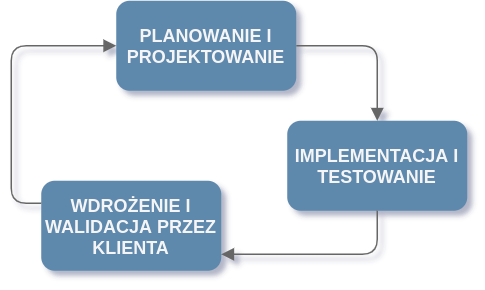
\includegraphics[scale=0.35]{agile.png}
\end{center}

Ryzyka projektowe są stale ewaluowane podczas każdej iteracji. Agile wprowadziło też ideę \textit{Proof of concept} - działający prototyp, który pozwala na dokładne badanie ryzyka wynikającego z proponowanych rozwiązań. Takie prototypy mogą być tworzone w dowolnym momencie pomiędzy iteracjami i to zespół decyduje, kiedy stworzenie \textit{PoC}\footnote{Skrót od Proof of concept} wprowadzi korzyści dla projektu.

Prototypy wcale nie muszą kończyć się powodzeniem - porażka może stanowić dla zespołu pewien rodzaj komunikatu, że wybrane przez nich rozwiązanie jest zbyt ryzykowne i zdecydować się na inne. \textit{PoC} często są do użytku wnętrznego, natomiast nic nie stoi na przeszkodzie prezentacja wyników klientowi - mogą one stanowić dowód trudności rozwiązań przez niego proponowanych i rozpozcąć dyskusję nad zmianą takich wymagań.

\subsubsection*{Zbieranie wymagań - User Stories jako nowe przypadki użycia}
Przypadki użycia z modelu kaskadowego były bardzo obszerne i mimo swojej złożoności czasami wcale nie dawały jawnego obrazu na to, jakie oczekiwania wobec niego mają odbiorcy. Informacje w nim przekazywane były zupełnie surowe - deweloperzy nie mieli okazji postawić się w roli użytkownika systemu, a analitycy spędzali większość czasu na budowaniu takich use case'ów, które pokryją dokładnie każdy scenariusz zachowania projektowanego systemu.

Zgodnie z hasłem "Działające produkty ponad złożoną dokumentacją" Agile zaproponowało alternatywny sposób zbierania wymagań - \textbf{User Stories}.

Zamiast długich przypadków użycia, User Stories mają być krótkie; ich forma wygląda następująco:

\begin{center}
    \textit{Jako \textbf{aktor}, chcę \textbf{wykonać czynność}, aby \textbf{osiągnąć pewien cel}.}
\end{center}

W odróżnieniu od przypadków użycia, które tworzone były przez analityków nie będącymi użytkownikami systemu, User Stories są tworzone we współpracy z klientem czy aktorami w systemie - ich prostota na to pozwala.

User stories stanowią najmniejszą jednostkę pracy dla zespołu.

\paragraph{Przykłady User Stories:}

\begin{center}
    Jako Pracownik che móc generować raporty, aby zwizualizować swoim klientom, szefowi lub kolegom z zespołu postępy, bądź informacje o postępach nad projektem.

    \paragraph{}
    Jako Użytkownik chce mieć możliwość zmiany danych osobowych w systemie na wypadek przeprowadzki, lub zmiany ważnych danych.

    \paragraph{}
    Jako Administrator potrzebuje funkcji zalogowania się jako inny użytkownik w systemie, aby diagnozować konkretne problemy napotkane przez tego użytkownika.

    \paragraph{}
    Jako Użytkownik chce móc edytować wysłane wiadomości na wypadek pomyłkek, literówek, żeby utrzymać jakość swoich wypowiedzi na wysokim poziomie

\end{center}

Ilość zrealizowanych User Stories na danym etapie projektu stanowi dobrą metrykę faktycznych postępów nad systemem. Reprezentują mierzalną wartość dla klienta, który podczas iteracji jest w stanie oceniać, czy są zrealizowane poprawnie.

\section{Metodyki zwinne}

\subsection{Scrum}
\subsubsection{Role w zespole}
\subsubsection{Organizacja pracy}

\subsection{Kanban}
\subsubsection{Tablica Kanbanowa}

\subsection{Scrumban}

\section{Proces w WMI Adventure}

\subsection{Metodyka}
\subsection{Role w zespole}
\subsection{User Stories}

\section{Wykorzystanie GitHub Projects jako narzędzia do zarządzania procesem}

\section{Ewolucja}

\end{document}
